\chapter{Winget}
\par
\section{O que é?}
O Winget, ou Windows Package Manager, é uma ferramenta de linha de comando para Windows que permite instalar, atualizar e gerenciar aplicativos de forma simples e eficiente. Ele foi desenvolvido pela Microsoft e é uma solução nativa para gerenciamento de pacotes no Windows.

Para maiores informações e entendimento veja a documentação em \cite{microsoft_winget}.
\par
\section{Porque usar nessa capacitação?}
Para que todos possam acompanhar de maneira eficaz essa capacitação, preciso que todos tenham as ferramentas git e GitHub CLI instaladas em suas máquinas. Para facilitar esse processo, utilizaremos o Winget, que é o gerenciador de pacotes nativo do Windows.
O Winget é um gerenciador de pacotes para Windows que facilita a instalação, atualização e remoção de aplicativos. Com ele, é possível automatizar a configuração do ambiente de desenvolvimento, economizando tempo e esforço.
\par
\subsection{Instalação}
\par
\begin{citacao}
A ferramenta de linha de comando do WinGet só tem suporte no Windows 10 versão 1809 (build 17763) ou posterior. 
O WinGet não estará disponível até que você tenha feito logon no Windows como usuário pela primeira vez, 
o que fará com que a Microsoft Store registre o Gerenciador de Pacotes do Windows como parte de um processo assíncrono. 
Se você tiver feito logon recentemente como usuário pela primeira vez e o WinGet ainda não estiver disponível, 
abra o PowerShell e insira o seguinte comando para solicitar o registro dele: 

\texttt{Add-AppxPackage -RegisterByFamilyName -MainPackage Microsoft.DesktopAppInstaller\_8wekyb3d8bbwe.}
\citeonline{microsoft_winget}.
\end{citacao}

\begin{enumerate}
  \item Verifique se o Winget já está instalado no seu sistema. Abra o Prompt de Comando ou PowerShell e digite
  \begin{verbatim}
    winget --version
  \end{verbatim}
  Se o comando retornar uma versão, o Winget já está instalado.
  \begin{figure}[H]
    \centering
    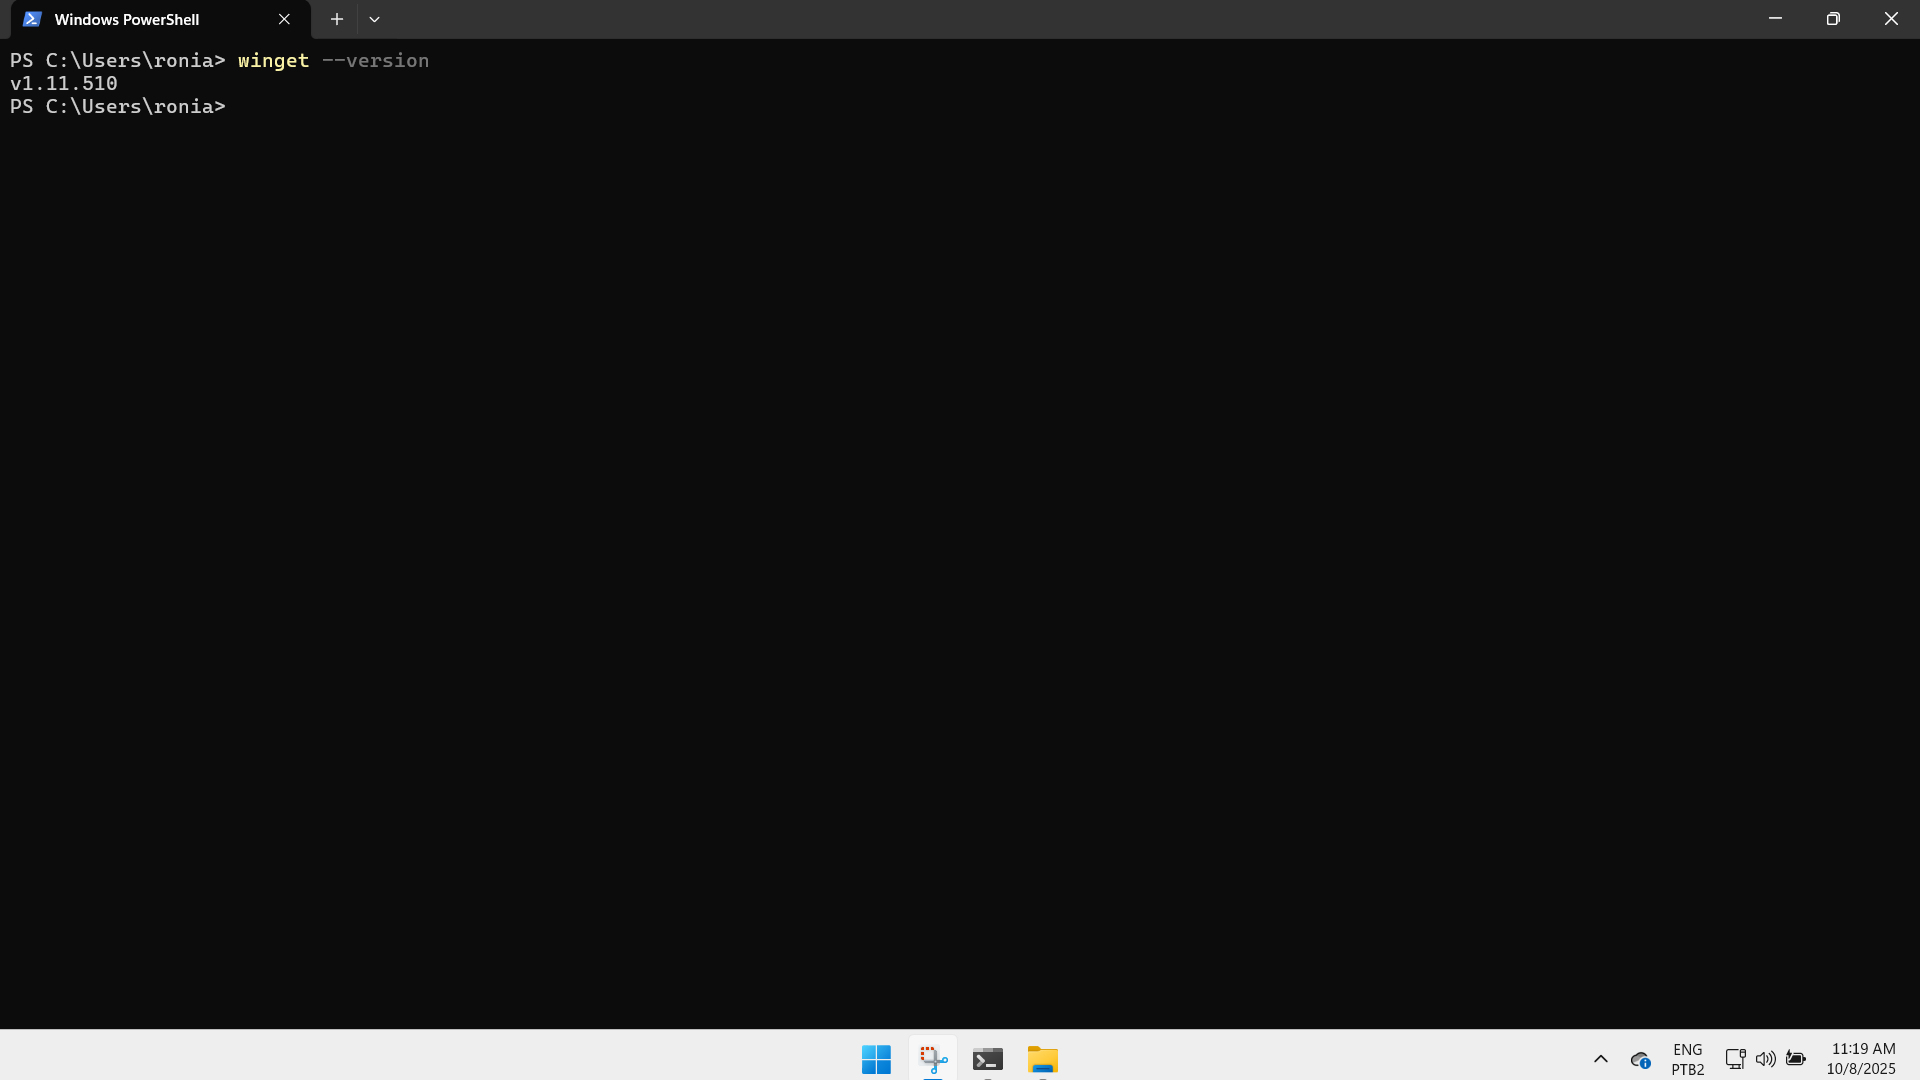
\includegraphics[width=0.9\textwidth]{./assets/images/07_winget_installed.png}
    \caption{Verificando se o Winget está instalado.}
    \label{fig:winget_installed}
  \end{figure}
  \item Caso o Winget não esteja instalado, você pode baixá-lo como parte do aplicativo "App Installer" da Microsoft Store. Acesse a Microsoft Store, procure por "App Installer" e clique em "Obter" para instalar. Caso enfrente alguma dificuldade, acesse a documentação em \cite{microsoft_winget}.
  \item Após a instalação, reinicie o Prompt de Comando ou PowerShell e verifique novamente a instalação com:
  \begin{verbatim}
    winget --version
  \end{verbatim}
  O comando deve retornar a versão do Winget instalada.
\end{enumerate}
\par
\subsubsection{Atualização}
Para garantir que você está utilizando a versão mais recente do Winget, execute o comando:
\begin{verbatim}
  winget upgrade --all
\end{verbatim}
Este comando atualizará todos os pacotes instalados, incluindo o próprio Winget, se houver uma atualização disponível.